\section{B.a.-ba des mathématiques}

\begin{frame}[fragile=singleslide]
  \frametitle{Principes de base}
  \begin{itemize}
  \item Décrire des équations mathématiques requiert un «langage» spécial
    \begin{itemize}
    \item il faut informer {\LaTeX} que l'on passe à ce langage
    \item par le biais de modes mathématiques
    \end{itemize}
  \item Important d'utiliser un mode mathématique
    \begin{itemize}
    \item règles de typographie spéciales
    \item espaces gérées automatiquement
    \end{itemize}
  \item Vous voulez utiliser le paquetage \pkg{amsmath}
\begin{lstlisting}
\usepackage{amsmath}
\end{lstlisting}
  \end{itemize}
\end{frame}

\begin{frame}[fragile]
  \frametitle{Modes mathématiques}
  \begin{enumerate}[<+->]
  \item «En ligne» directement dans le texte comme $(a + b)^2 = a^2 +
    2ab + b^2$ en plaçant l'équation entre \verb=$ $=
\begin{lstlisting}
«En ligne» directement dans le texte
comme $(a + b)^2 = a^2 + 2ab + b^2$
\end{lstlisting}
  \item «Hors paragraphe» séparé du texte principal comme
    \begin{equation*}
      \int_0^\infty f(x)\, dx = \sum_{i = 1}^n \alpha_i e^{x_i} f(x_i)
    \end{equation*}
    en utilisant divers types d'environnements
\begin{lstlisting}
«Hors paragraphe» séparé du texte principal comme
\begin{equation*}
  \int_0^\infty f(x)\, dx =
  \sum_{i = 1}^n \alpha_i e^{x_i} f(x_i)
\end{equation*}
\end{lstlisting}
  \end{enumerate}
\end{frame}


\begin{conseil}
  En ligne ou hors paragraphe, les équations font partie intégrante de
  la phrase.

  Les règles de ponctuation usuelles s'appliquent donc aux équations.

  \bigskip
  \fbox{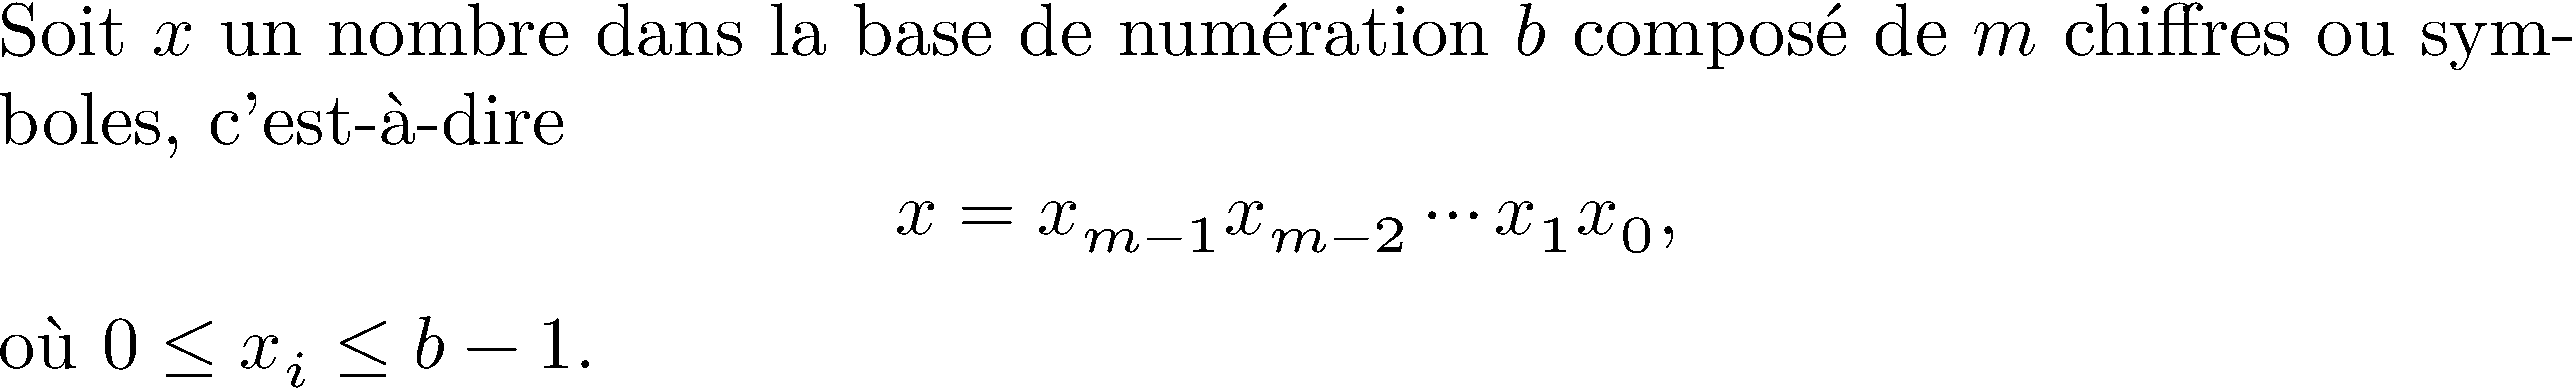
\includegraphics[width=0.95\linewidth]{ponctuation}}
\end{conseil}

\begin{frame}[fragile]
  \frametitle{Quelques règles de base}
  \begin{itemize}
  \item En mode mathématique, {\TeX} écrit automatiquement les
    constantes en romain et les variables en italique
    \begin{demo}
      \begin{texample}
\begin{lstlisting}
$z = 2a + 3y$
\end{lstlisting}
        \producing
        $z = 2a + 3y$
      \end{texample}
    \end{demo}
  \item Espacement entre les éléments géré automatiquement, peu importe
    le code source
    \begin{demo}
      \begin{texample}
\begin{lstlisting}
$z=2 a+3 y$
\end{lstlisting}
        \producing
        $z=2 a+3 y$
      \end{texample}
    \end{demo}
  \end{itemize}
\end{frame}

\begin{frame}[fragile]
  \frametitle{Quelques règles de base (suite)}
  \begin{itemize}
  \item \alert{Ne pas} utiliser le mode mathématique pour obtenir du
    texte en italique!
    \begin{demo}
      \begin{minipage}{0.45\linewidth}
\begin{lstlisting}
\emph{xyz}
\end{lstlisting}
      \end{minipage}
      \hfill
      \begin{minipage}{0.45\linewidth}
        
\includegraphics[height=0.8\baselineskip,keepaspectratio]{xyz-emph}
      \end{minipage}\par
      \begin{minipage}{0.45\linewidth}
\begin{lstlisting}
$xyz$
\end{lstlisting}
      \end{minipage}
      \hfill
      \begin{minipage}{0.45\linewidth}
        
\includegraphics[height=0.8\baselineskip,keepaspectratio]{xyz-math}
      \end{minipage}
    \end{demo}
  \item Commande \cs{text} de \pkg{amsmath} pour texte à
    l'intérieur du mode mathématique
    \begin{demo}
      \begin{texample}
\begin{lstlisting}
$x = 0 \text{ si } y < 2$
\end{lstlisting}
        \producing
        $x = 0 \text{ si } y < 2$
      \end{texample}
    \end{demo}
  \end{itemize}
\end{frame}

\begin{frame}[fragile]
  \frametitle{Avant-goût}

  Pouvez-vous interpréter ce code?
\begin{lstlisting}
\begin{equation*}
  \Gamma(\alpha) =
  \sum_{j = 0}^\infty \int_j^{j + 1}
    x^{\alpha - 1} e^{-x}\, dx
\end{equation*}
\end{lstlisting}
  \vspace{18pt}
  \pause

  Fort probablement!
  \begin{equation*}
    \Gamma(\alpha) =
    \sum_{j = 0}^\infty \int_j^{j + 1} x^{\alpha - 1} e^{-x}\, dx
  \end{equation*}
\end{frame}

%%% Local Variables:
%%% TeX-master: "formation-latex-ul-diapos"
%%% TeX-engine: xetex
%%% coding: utf-8
%%% End:
